\documentclass[tikz,margin=3.14mm]{standalone}
\usepackage{tikz}

\usepackage{pgfplots}
\usepackage{pgfplotstable}
\usepgfplotslibrary{groupplots}
\usepackage{amsmath, amssymb, amsfonts}

\usetikzlibrary{arrows, decorations}

\pgfplotsset{compat=1.18}


\pgfdeclarelayer{background}% determine background layer
\pgfsetlayers{background,main}% order of layers

\begin{document}
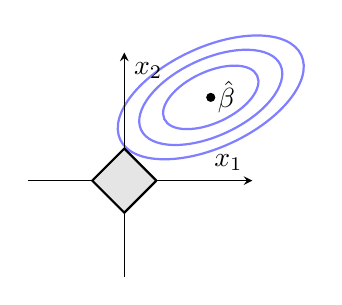
\begin{tikzpicture}

\begin{axis}[
    xlabel={$x_1$},
    ylabel={$x_2$},
    xmin=-1.5, xmax=2,
    ymin=-1.5, ymax=2,
    xtick={0},
    ytick={0},
    grid=both,
    grid style={line width=.1pt, draw=gray!10},
    major grid style={line width=.2pt,draw=gray!50},
    axis lines=middle,
    samples=100,
    clip mode = individual,
    clip = false,
    scale = .5,
    width=.6\textwidth,
    height=.6\textwidth,
]

    % LASSO
    \coordinate (betahat) at (axis cs: 1.35,1.3);
    \node[circle, 
          inner sep = 0pt, 
          minimum size = .5mm, 
          fill = black, 
          scale=.5] at (betahat) {a};
          
    \node[xshift=2mm] at (betahat) {$\hat \beta$}; % label for the regression coefficient

    \begin{pgfonlayer}{background}
    % concentric ellipses of uncertainty around \hat \beta 
    \draw[blue, thick, opacity = .5] (betahat) ellipse [x radius=0.4, y radius=.8, rotate = -65];
    \draw[blue, thick, opacity = .5] (betahat) ellipse [x radius=0.6, y radius=1.2, rotate = -65];
    \draw[blue, thick, opacity = .5] (betahat) ellipse [x radius=.78, y radius=1.56, rotate = -65];    
    \end{pgfonlayer}

    % the region within the LASSO constraint
    \draw [thick, fill = gray!20] (axis cs: 0.5, 0) -- (axis cs: 0, 0.5) -- 
      (axis cs: -.5, 0) -- (axis cs: 0, -.5) -- (axis cs: 0.5, 0);
    
    \end{axis}
\end{tikzpicture}
\end{document}
